\section{Auswertung}
\label{sec:Auswertung}

\subsection{Fehlerrechnung}
Durch die angegebenen relativen Fehler der Bauteile ist die Gauß'sche Fehlerfortpflanzung für Größen der Form
\begin{align*}
  z = x \cdot y    
\end{align*}
zu
\begin{align*}
  \Delta z = \bar{z}\sqrt{(\Delta x)^2 + (\Delta y)^2}    
\end{align*}
zu bestimmen, wobei $\bar{z}$ der Mittelwert und $\Delta x$ und $\Delta y$ die relativen Fehler sind.


\subsection{Wheatstone'sche Messbrücke}
%Daten Aufgabenteil a)
In \autoref{tab:wertea} sind die Messwerte für die Wheatstone'sche Messbrücke aufgeführt.
\begin{table}[H]
  \centering
  \caption{Messwerte zur Wheatstone Messbrücke.}
  \label{tab:wertea}
  \begin{tabular}{c c c c}
    \toprule
    $R_{\text{x}}$ & $R_{\text{2}} \:/\: \upOmega$ & $R_{\text{3}} \:/\: \upOmega$ & $R_{\text{4}} \:/\: \upOmega$ \\
    \midrule
    Wert 10 & 500 & 327 & 673 \\
    Wert 10 & 1000 & 196 & 804 \\
    Wert 13 & 500 & 393,5 & 606,5 \\
    Wert 13 & 1000 & 245,5 & 754,5 \\
    \bottomrule
  \end{tabular}
\end{table}
Die baubedingten relativen Fehler der Widerstände lauten für $R_2$ 0,2\% und für das Verhältnis $\frac{R_3}{R_4}$ 0,5\%. Mit den Werten aus \autoref{tab:wertea} und
Formel \autoref{eqn:wheatstoneGleichung} lassen sich nun die Widerstände $R_x$ mit Wert 10 und Wert 13 bestimmen.
\begin{align*}
  R_{10} &= 243,36 \pm 0,5940 \upOmega \\
  R_{13} &= 324,89 \pm 0,6930 \upOmega \\
\end{align*}
Die relativen Fehler betragen somit
\begin{align*}
  \Delta R_{10} &= 1,31 \upOmega , \\
  \Delta R_{13} &= 1,75 \upOmega . \\
\end{align*}

\subsection{Kapazitätsmessbrücke}
% Daten Aufgabenteil b)
Aus \autoref{tab:werteb} sind die Messwerte zur Kapazitätsmessbrücke zu entnehmen.
\begin{table}[H]
  \centering
  \caption{Messwerte zur Kapazitätsmessbrücke.}
  \label{tab:werteb} 
  \begin{tabular}{c c c c c c}
    \toprule
    $R_{\text{x}}$ & $C_{\text{x}}$ & $R_{\text{2}} \:/\: \upOmega$ & $C_{\text{2}} \:/\: \si{\nano\farad}$ & $R_{\text{3}} \:/\: \upOmega$ & $R_{\text{4}} \:/\: \upOmega$ \\
    \midrule
    Wert 9 & Wert 9 & 99 & 994 & 995 & 5 \\
    Wert 9 & Wert 9 & 99 & 399 & 785 & 215 \\
    \bottomrule
  \end{tabular}
\end{table}
Der relative Fehler von $R_2$ ist hier als 3\% und der von $C_2$ als 0,2\% anzunehmen. Mit Hilfe von \autoref{eqn:kapazitaetsmess} und \autoref{eqn:wheatstoneGleichung} und den
Werten aus \autoref{tab:werteb} lassen sich nun $R_x$ und $C_x$ bestimmen zu
\begin{align*}
  R_x &= 361,47 \upOmega \\
  C_x &= 109,28 \si{\nano\farad} \\
\end{align*}
mit relativen Fehlern
\begin{align*}
  \Delta R_x &= 10,87 \upOmega \\
  \Delta C_x &= 3,29 \si{\nano\farad} . \\
\end{align*}


\subsection{Induktivitätsmessbrücke}
% Daten Aufgabenteil c)
In \autoref{tab:wertec} sind die Messwerte zur Induktivitätsmessbrücke aufgetragen.
\begin{table}[H]
  \centering
  \caption{Gemessene Messwerte zu Aufgabenteil c).}
  \label{tab:wertec}
  \begin{tabular}{c c c c c c}
    \toprule
    $R_{\text{x}}$ & $L_{\text{x}}$ & $R_{\text{2}} \:/\: \upOmega$ & $L_{\text{2}} \:/\: \si{\milli\henry}$ & $R_{\text{3}} \:/\: \upOmega$ & $R_{\text{4}} \:/\: \upOmega$ \\
    \midrule
    Wert 18 & Wert 18 & 474 & 20,1 & 480 & 520 \\
    Wert 18 & Wert 18 & 475 & 14,6 & 500 & 500 \\
    \bottomrule
  \end{tabular}
\end{table}
Die relativen Fehler für das Potentiometer und für $R_2$ sind identisch wie vorher, der für $L_2$ ist gegeben als 0,2\%
Mit den Formeln \autoref{eqn:wheatstoneGleichung} und \autoref{eqn:induktivitaetsmess} und den Messwerten aus \autoref{tab:wertec} werden nun $R_{\text{x}}$
und $L_{\text{x}}$ bestimmt.
\begin{align*}
  R_x &= 456,27 \pm 26,49 \upOmega \\
  L_x &= 18,19 \pm 5,08 \si{\milli\henry} . \\
\end{align*}
Diese Größen besitzen die relativen Fehler
\begin{align*}
  \Delta R_x &= 0,045 \upOmega \\
  \Delta L_x &= 0,0018 \si{\nano\farad} . \\
\end{align*}


\subsection{Maxwellbrücke}
% Daten Aufgabenteil d)
Aus \autoref{tab:werted} sind die Messwerte zur Maxwellbrücke zu entnehmen.
\begin{table}[H]
  \centering
  \caption{Gemessene Messwerte zu Aufgabenteil d).}
  \label{tab:werted}
  \begin{tabular}{c c c c c c}
    \toprule
    $R_{\text{x}}$ & $L_{\text{x}}$ & $R_{\text{2}} \:/\: \upOmega$ & $R_{\text{3}} \:/\: \upOmega$ & $R_{\text{4}} \:/\: \upOmega$  & $C_{\text{4}} \:/\: \si{\nano\farad}$ \\
    \midrule
    Wert 18 & Wert 18 & 1000 & 91 & 240 & 750 \\
    Wert 18 & Wert 18 & 500 & 101 & 113 & 750 \\
    \bottomrule
  \end{tabular}
\end{table}
Die relativen Fehler für $R_3$ und $R_4$ sind angegeben als 3\%, die für $R_2$ und $C_2$ als 0,2\%. Mit Hilfe von Formel \autoref{eqn:wheatstoneGleichung} und
\autoref{eqn:maxwellgl} und den Werten aus \autoref{tab:werted} können $R_{\text{x}}$ und $L_{\text{x}}$ zu
\begin{align*}
  R_x &= 413,04 \upOmega \\
  L_x &= 52.687,5 \si{\nano\farad} . \\
\end{align*}
mit relativen Fehlern
\begin{align*}
  \Delta R_x &= 12,42 \upOmega \\
  \Delta L_x &= 1584,13 \si{\nano\farad} . \\
\end{align*}
bestimmt werden.


\subsection{Wien-Robinson-Brücke}
% Daten Aufgabenteil e)
Zur Untersuchung der Frequenzabhängigkeit der Brückenspannung wird der Quotient der effektive Brückenspannung $U_{\text{Br}}$ und der Speisespannung $U_{\text{S}}$
gegen $\frac{f}{f_0}$ aufgetragen(\autoref{fig:plot}). Zusätzlich wird eine Theoriekurve eingefügt, die sich aus Formel \autoref{eqn:theo} ergibt.

In \autoref{tab:wertee} sind die Messwerte zur Wien-Robinson-Brücke aufgetragen. Die Bauteile der Schaltung haben die Werte
\begin{align*}
  C = \SI{660}{\nano\farad},\\
  R = \SI{1000}{\ohm}, \\
  R' = \SI{332}{\ohm}, \\
  U_{\text{S}} = \SI{1}{\volt}. \\
\end{align*}

\begin{table}[H]
  \centering
  \caption{Gemessene Messwerte zu Aufgabenteil e).}
  \label{tab:wertee}
  \begin{tabular}{c c}
    \toprule
    Frequenz $\,/\,\si{\hertz}$ &  $U\,/\, \si{\milli\volt}$ \\
    \midrule
    20 & 300 \\
    40 & 280 \\
    80 & 210 \\
    160 & 75 \\
    180 & 50 \\
    200 & 34 \\
    220 & 16 \\
    230 & 7 \\
    235 & 5 \\
    240 & 0 \\
    245 & 5 \\
    250 & 7 \\
    260 & 15 \\
    280 & 30 \\
    300 & 45 \\
    320 & 60 \\
    340 & 65 \\
    640 & 17 \\
    1280 & 250 \\
    2560 & 250 \\
    5120 &  250 \\
    10240 & 250 \\
    20480 & 200 \\
    30000 & 140 \\
    \bottomrule
  \end{tabular}
\end{table}

\begin{figure}
  \centering
  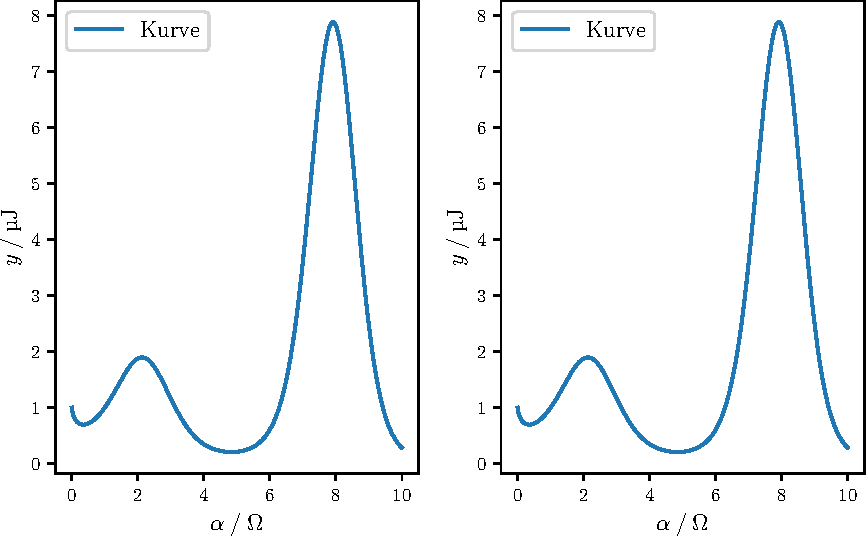
\includegraphics{plot.pdf}
  \caption{Messdaten und Theoriekurve}
  \label{fig:plot}
\end{figure}

Zur bestimmung des Klirrfaktor werden nun $U_2$ und $U_1$ benötigt. Da $U_1$ als $U_{\text{S}}$ bei $f_0$ gegeben ist, muss lediglich $U_2$ durch

\begin{align*}
  U_2 &= \frac{0,32\si{\volt}{\sqrt{\frac{(2^2 - 1)^2}{9((1-2^2)^2 + 9 \cdot 2^2)}}} \\
  &= 2,1466 \si{\volt}
\end{align*}

Der Klirrfaktor ergibt sich somit Zu
\begin{align*}
  k = \frac{U_2}{U_1} = 2,1466 \\
\end{align*}

\begin{figure}
  \centering
  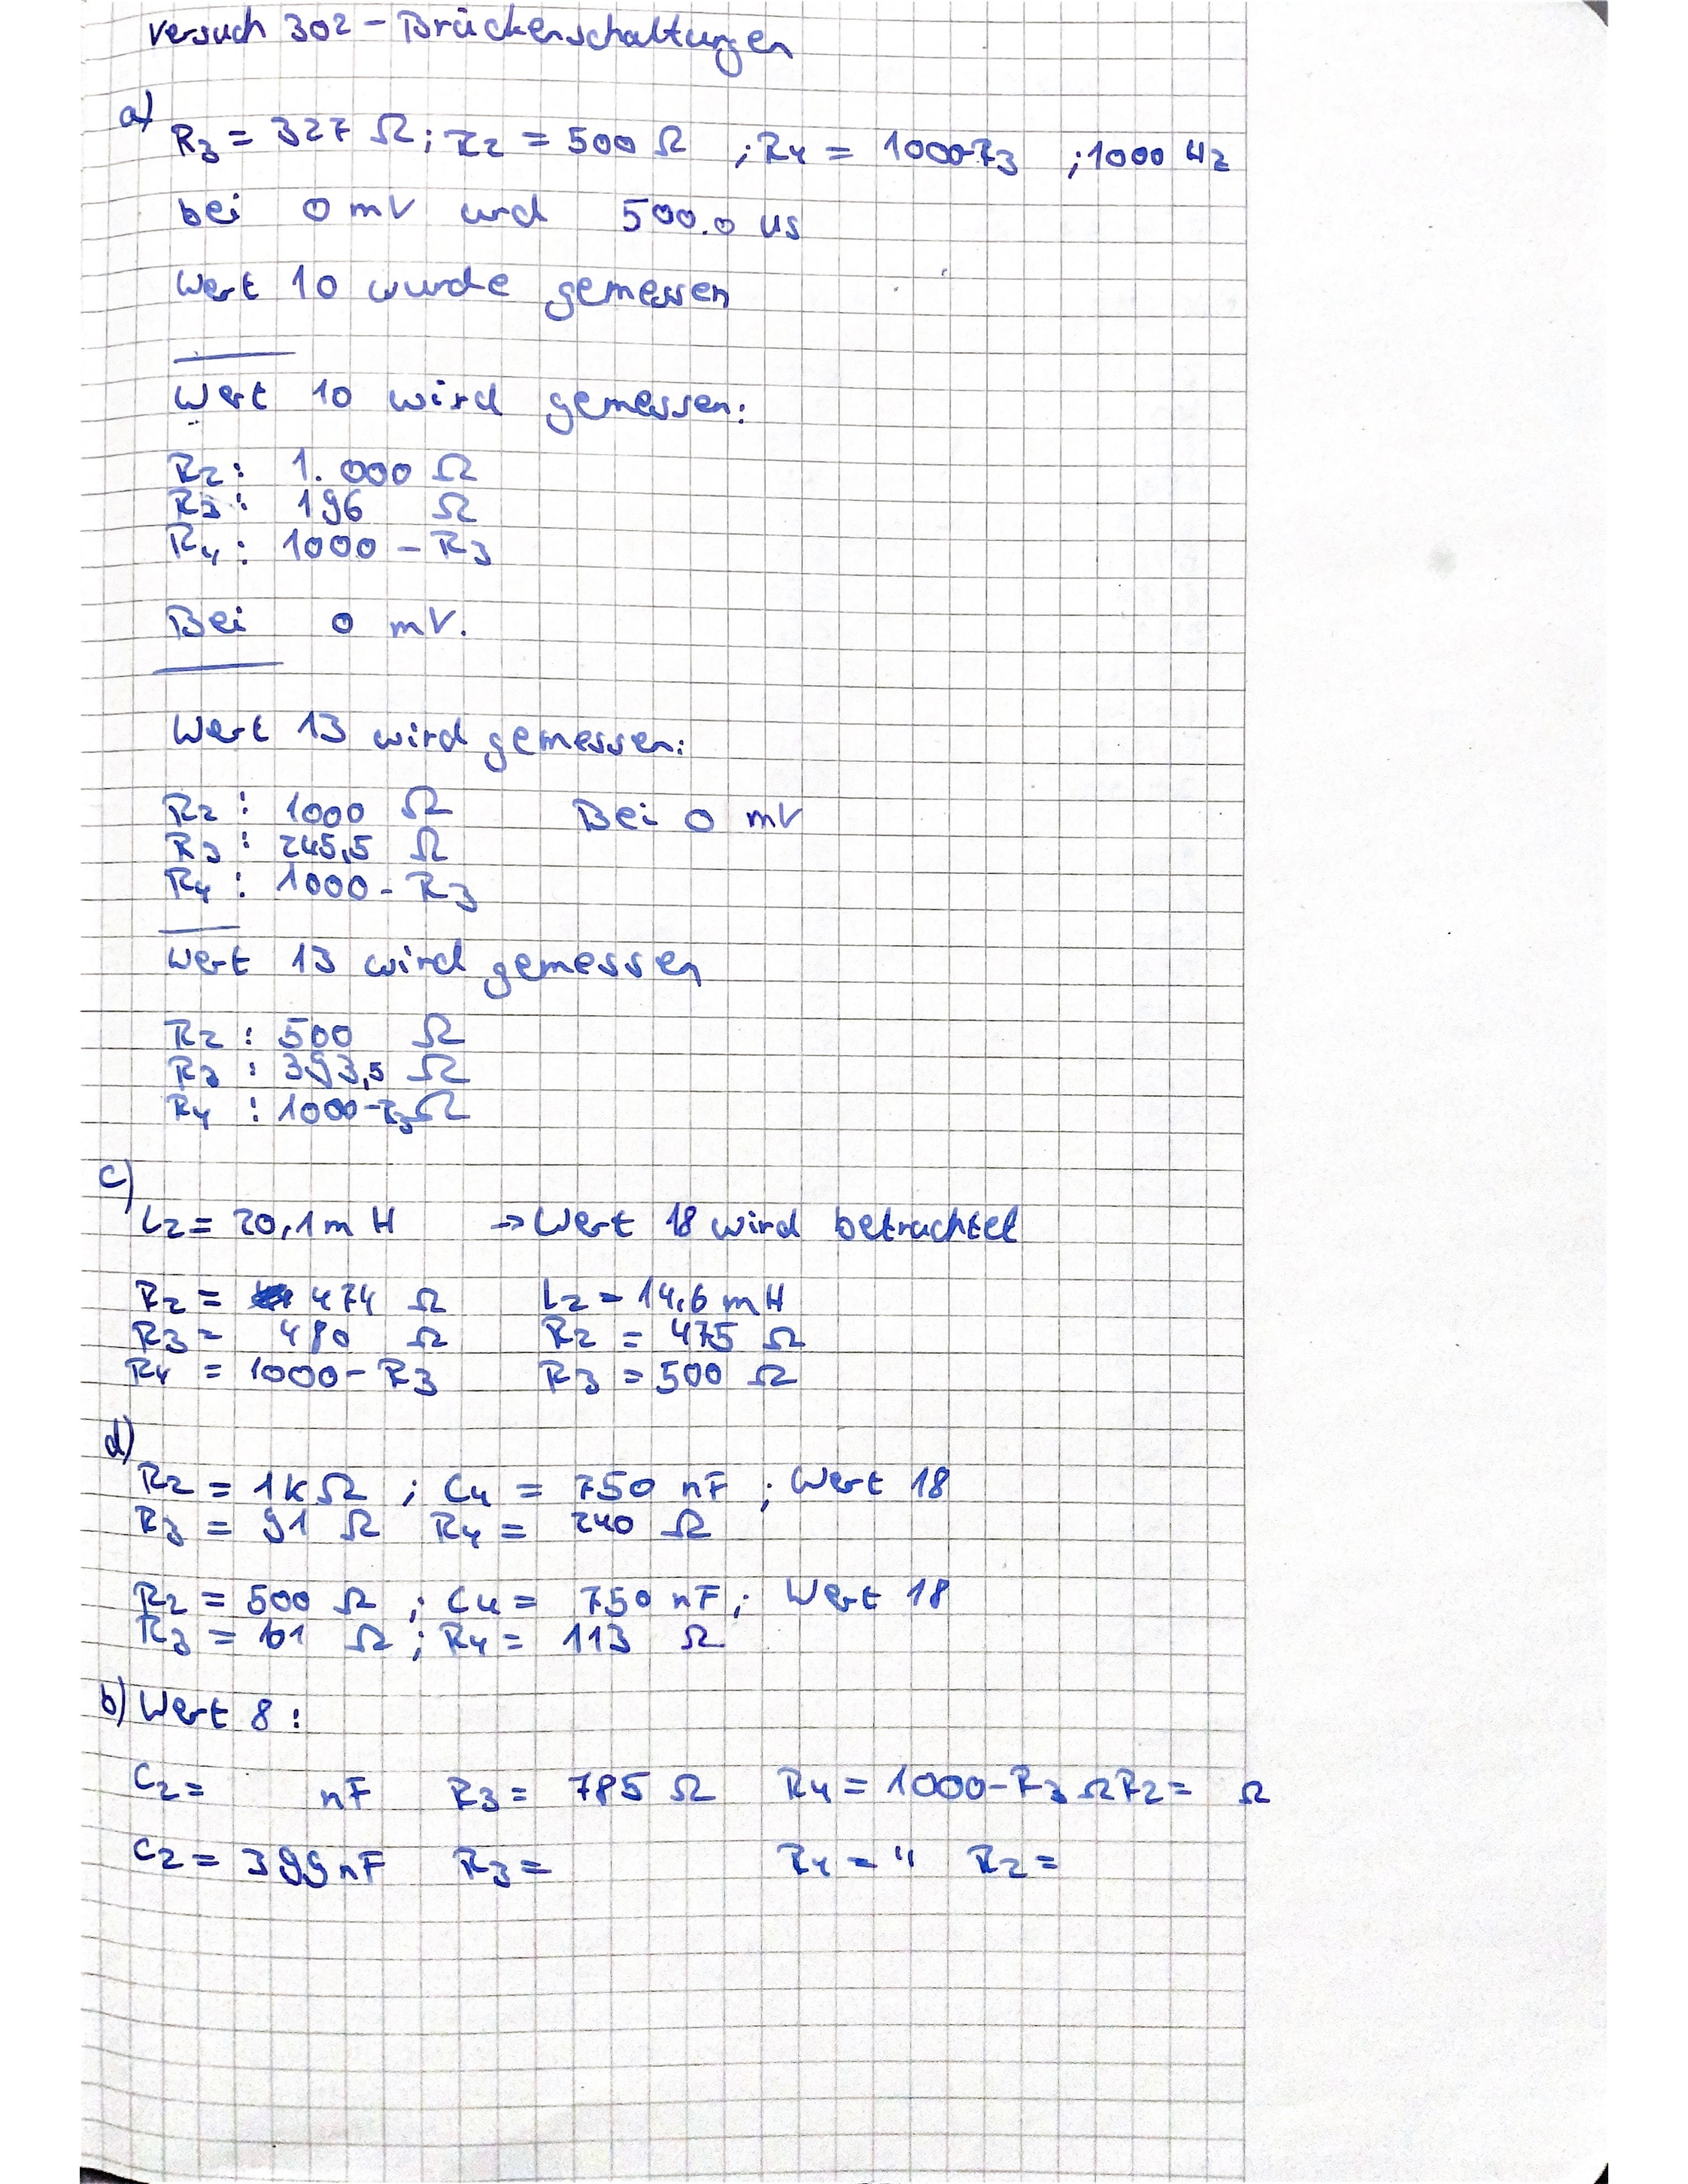
\includegraphics[width=0.75\textwidth]{dateien/daten1.jpg}
  \caption{Originale Messdaten.}
  \label{fig:daten1}
\end{figure}

\begin{figure}
  \centering
  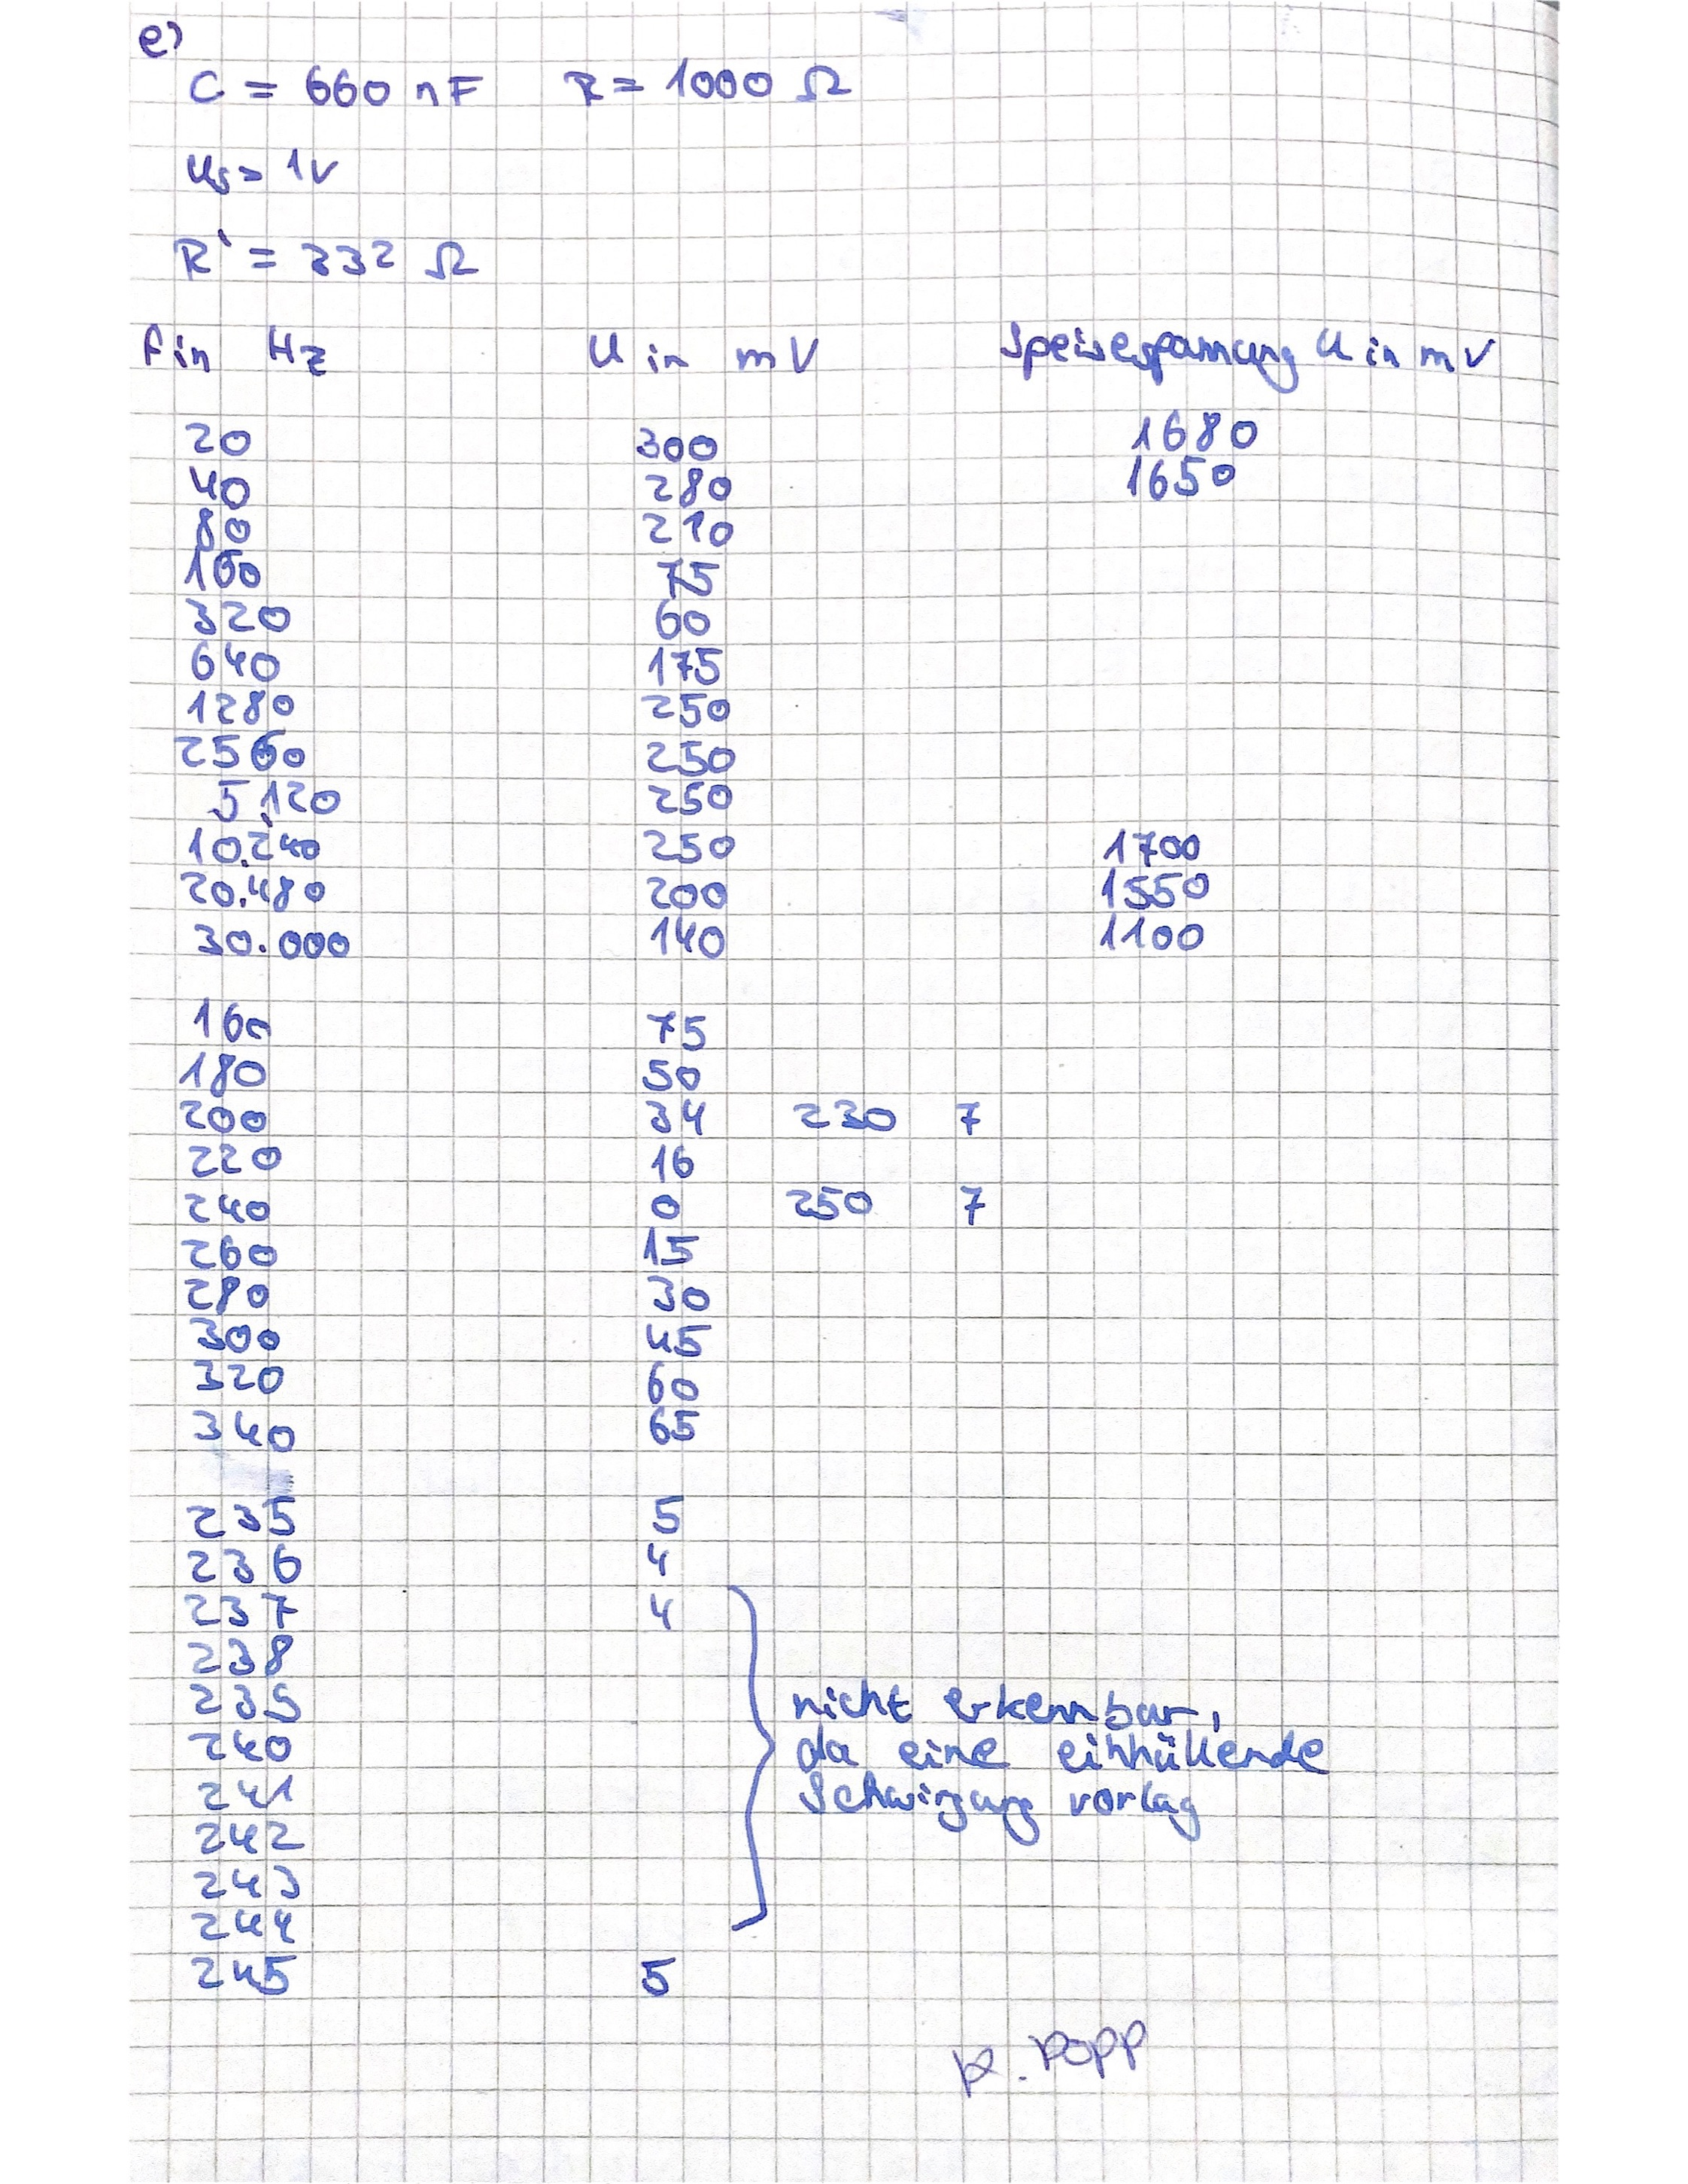
\includegraphics[width=0.75\textwidth]{dateien/daten2.jpg}
  \caption{Originale Messdaten.}
  \label{fig:daten2}
\end{figure}